\chapter{Aspectos conceituais}
\label{CAP2}


A seguir serão explicados os conceitos fundamentais que possibilitam a execução deste trabalho. 


\section{Efeito Estroboscópico}

O efeito estroboscópico será a base de funcionamento do projeto. Descoberto na decadá de 1830, o efeito consiste do uso de diferentes técnicas para a captura de um movimento continuo ou cíclico com um taxa de amostragem feita de tal maneira que o  movimento aparente é nulo.

Nesse projeto, será usado um variação especifico do efeito conhecida como efeito da roda-de-carroça (\textit{Wagon-wheel effect}) \cite{tessive}. O nome é originado dos filmes de faroeste em que as rodas das carroças pareciam se mover no sentido oposto a que era esperado.

O efeito da roda-de-carroça  acontece quando a taxa de quadros por segundo na câmera é um múltiplo do período de rotação de um objeto, fazendo-o parecer parado, se movimentando devagar ou num sentido inesperado. 

O efeito pode ter vários usos práticos como para a calibração da velocidade de um disco de vinil ou para maquinário pesado.


\begin{figure}[H]
    \centering
    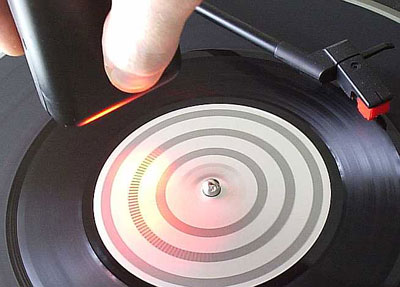
\includegraphics[width=0.8\textwidth,angle=0]{figures/strobe_3.jpg}
    \caption{Demonstração do efeito estroboscópico sobre um disco de vinil}
\end{figure}

\begin{figure}[H]
    \centering
    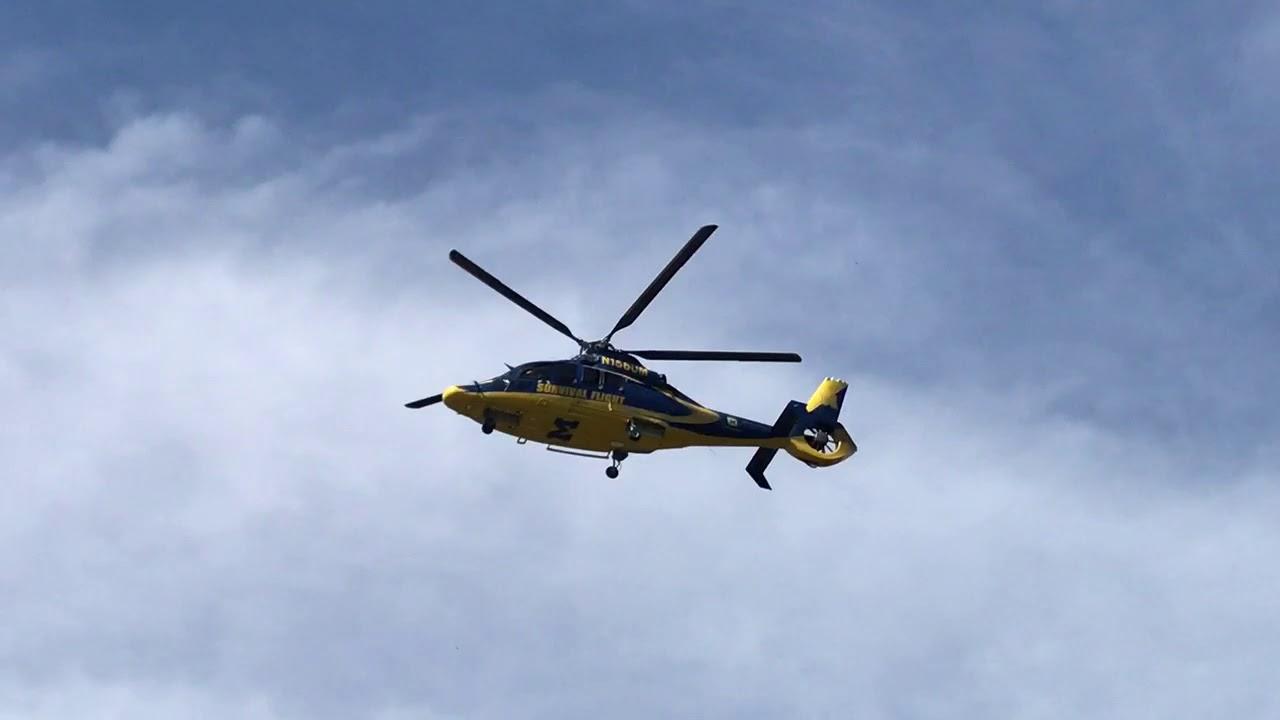
\includegraphics[width=0.8\textwidth,angle=0]{figures/helicoptero_parado.jpg}
    \caption{O rotor do helicóptero parece parada graças ao efeito roda-de-carroça }
\end{figure}
\pagebreak

\section{\textit{Motion Blur}}

\textit{Motion Blur} (borrar imagem em movimento), ocorre quando um objeto se movimenta durante o período de exposição de uma fotografia. 

O blur é benéfico em muitas situações, pode fazer o movimento rapido de umobjeto parecer mais suave, mas para o caso de camera de mover existem dois problemas: 


primeiramente a imagem pode ficar completamente borrada, segundamente nas cameras mais simples como as de celulares, o blur pode confundir o sistema de foco automatico e acaba por gerar uma imagem borrada, mesmo com exposições baixas. 

\begin{figure}[H]
    \centering
    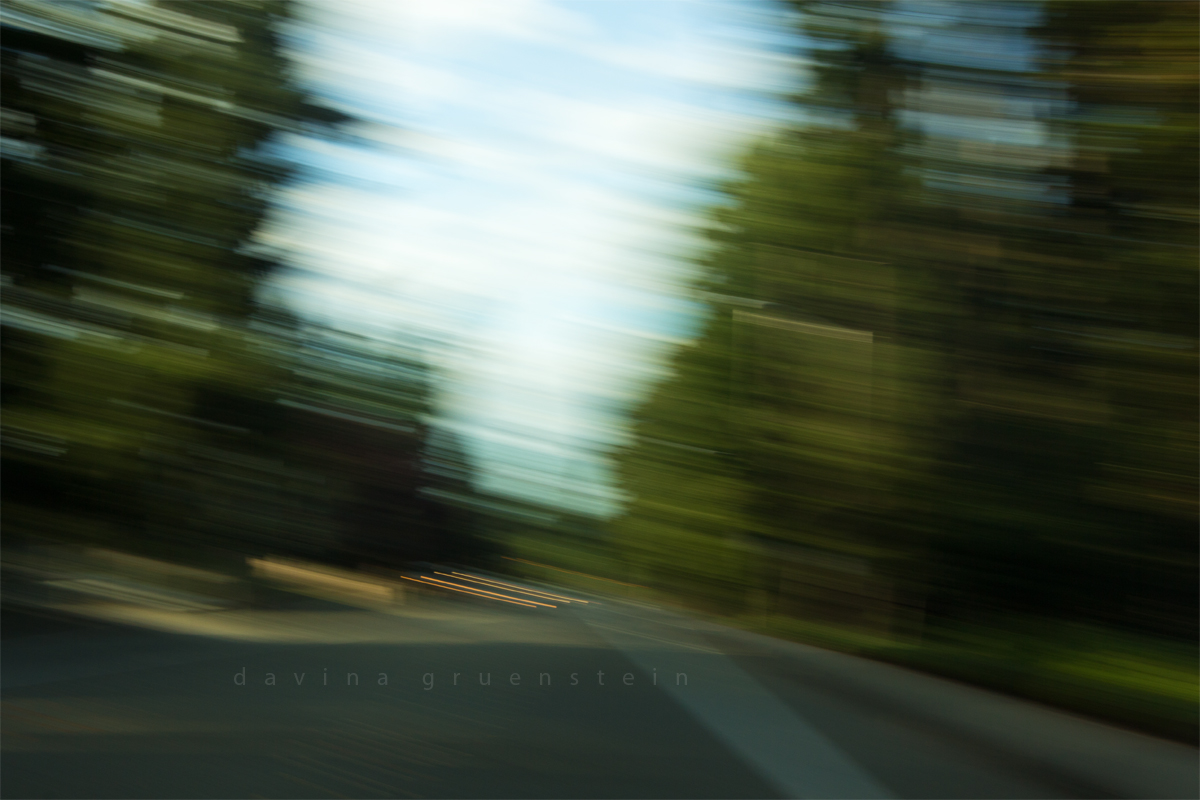
\includegraphics[width=0.9\textwidth,angle=0]{figures/motion-blur3.jpg}
    \caption{Imagem borrada deviado a motion blur. Imagem de: Davina Gruenstein}
\end{figure}